
\section{Solution development}

%\subsection{Requirements}\


%Identify the relevant functional and non-functional requirements and their sources, as well as project constraints.
%\begin{itemize}
 %   \item Functional requirements
    
%    - a
%    \item Non-functional requirements
    
%    -a
%    \item Project constraints
    
%    -a
%\end{itemize}





%\subsection{Overview}

%\subsubsection{VizML}
%VizML is a machine learning approach that uses deep neural networks to recommend visualizations. It processes dataset features and predicts the most suitable chart type through a fully connected feedforward neural network. The system is trained on dataset-visualization pairs extracted from the Plotly Community Feed, focusing on accuracy and scalability.
%\subsubsection{KG4Vis}
%KG4Vis is a knowledge graph-based approach that models relationships between dataset features and visualization choices using TransE embeddings. It emphasizes explainability and flexibility, allowing for dynamic expansion of the knowledge graph without retraining. The method builds on the VizML dataset but structures the data as a graph for inference-based recommendations.


\subsection{Approach}
According to [1] and [2]:
\begin{itemize}
\item VizML is a machine learning approach that uses deep neural networks to recommend visualizations. It processes dataset features and predicts the most suitable chart type through a fully connected feedforward neural network. The system is trained on dataset-visualization pairs focusing on accuracy and scalability.

\item KG4Vis is a knowledge graph-based approach that models relationships between dataset features and visualization choices using TransE embeddings. It emphasizes explainability and flexibility, allowing for dynamic expansion of the knowledge graph without retraining. The method builds on the VizML dataset but structures the data as a graph for inference-based recommendations. 
\end{itemize}

All this is illustrated in Fig. 1.


\vspace{0.1cm}



\begin{figure}[h]
    \centering
    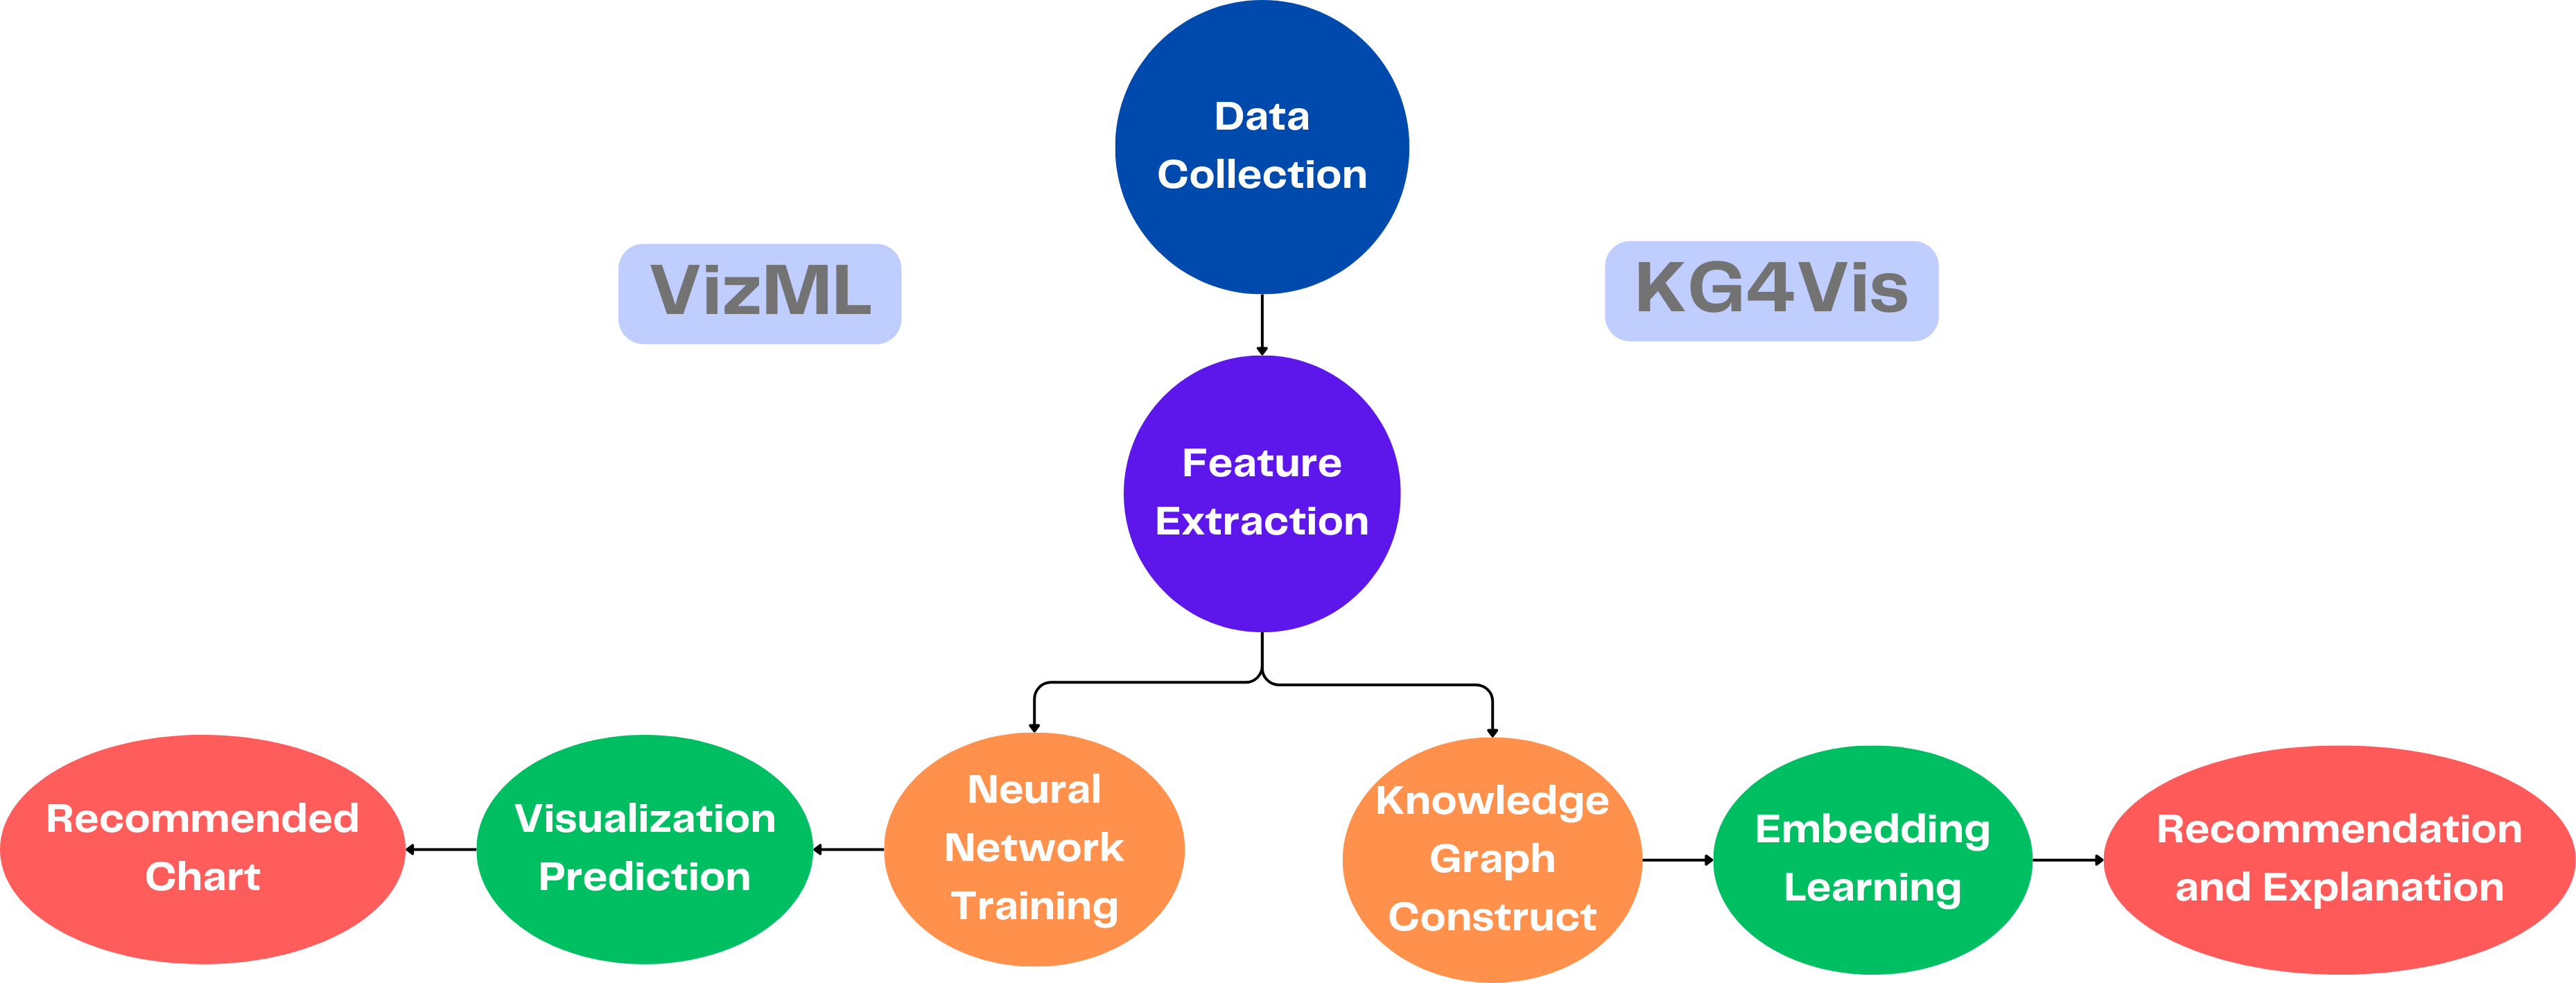
\includegraphics[width=1\textwidth]{Pipeline_VizML_KG4Vis.png}
    \caption{Pipeline of VizML and KG4Vis.}  
    \label{fig:pipelineVizMLKG4Vis}               
\end{figure}
\vspace{0.3cm}
\begin{itemize}
\item Both models rely on a large dataset of dataset-visualization pairs, and both typically get their data from Plotly (KG4Vis gets it from VizML which gets it from Plotly).

\end{itemize}
We also found that, when extracting, the goal is to quantify the characteristics of the dataset to help select the right representation, with VizML extracting numerical features, such as statistical properties (mean, variance, etc.) and structural attributes (number of columns, missing values, etc.), and KG4Vis encoding the features as nodes in a knowledge graph.

\subsubsection{VizML}
According to [1]:
\begin{itemize}
\item VizML uses a supervised deep learning model, which means that it learns from labeled dataset-visualization pairs.
It processes 841 extracted features per dataset and gives them to a fully connected neural network.
The goal is for the network to map dataset features to the best-fitting visualization type.

\item As mentioned above, VizML makes use of PyTorch to turn dataset features into sensors, which then allows the network to learn by minimizing prediction error, by adjusting weights through backpropagation.

\item This process is done in small batches to improve efficiency, but even so it is computationally expensive, often requiring larger RAM and VRAM capacity and GPU acceleration, for example, to handle large datasets.

\end{itemize}



We also found that once the model has finished training, it can predict the most suitable visualization type in real time using a dataset’s feature vector in a single forward pass through the network, resulting in fast inference.
This, however, reduces its explainability, as it quickly gives an answer but does not justify or elaborate it.


\newcommand{\lowtilde}{\raisebox{-0.5ex}{\textasciitilde}} % Lower the tilde

\subsubsection{KG4Vis}
According to [2]:
\begin{itemize}
    \item KG4Vis builds knowledge graphs with the extracted features, with the nodes representing the dataset attributes, visualization types and encoding choices, and the edges defining meaningful relations, for example, categorical data being best represented by a bar chart (“Categorical data ——— Bar Char”). This makes it dynamically expandable, meaning it can receive and integrate new dataset features and/or visualization types without retraining and starting again from the beginning. It also helps with interpretability, since all relations are explicitly defined.

\item KG4Vis learns vector representations (embeddings) for each node and relation in the knowledge graph. It uses TransE embeddings, which dictate that if A and B are related by R, then in vector space A~+~R~\lowtilde\lowtilde~B.
Pytorch is used in this case to help train these embeddings, as mentioned before, by helping to compute and update the knowledge graphs, so the model can predict possible missing links from it.
The embedding space preserves the relationships between data and visualization types, which helps explainability.
\end{itemize}

We also found that KG4Vis, instead of directly predicting, instead retrieves the most relevant visualization based on its learned knowledge graph structure post-training.
Due to the nature of the graph, it can then trace back the recommendation, allowing it to explain why that particular visualization is suitable, offering better explainability.





\subsection{Technical Implementation}

\subsubsection{Neural Network Training (VizML)}

According to [1]:
\begin{itemize}
\item VizML employs a fully connected feedforward neural network (NN) as its primary model, implemented using the PyTorch framework. The network architecture consists of three hidden layers, each containing 1,000 neurons with Rectified Linear Unit (ReLU) activation functions. ReLU was selected because of its computational efficiency, ability to mitigate the vanishing gradient problem, and tendency to induce sparse activations, which can improve model generalization.

\item The training process utilizes the Adam optimizer with a mini-batch size of 200 and an initial learning rate of $5 \times 10^{-4}$. To optimize convergence, a dynamic learning rate scheduling mechanism is employed: the learning rate is reduced by a factor of 10 whenever the validation accuracy fails to improve beyond a threshold of $10^{-3}$ over a span of 10 epochs. Training terminates either after the third learning rate reduction or upon reaching 100 epochs, whichever occurs first. Empirical evaluations indicated that additional regularization techniques, such as weight decay, dropout, and batch normalization, did not yield significant performance improvements, suggesting that the baseline architecture already achieves sufficient generalization without further constraints.
\end{itemize}

\paragraph{Neural Network Topology}
The network follows a sequential feedforward structure, where each layer is fully connected to the subsequent one, and the information propagates unidirectionally from input to output without cyclic loops. The architecture comprises:

\begin{itemize}
    \item Input Layer: The dimensionality of this layer is determined by the size of feature set, serving as the initial representation of the input data.
    \item Hidden Layers: Three intermediate layers, each with 1,000 neurons and ReLU activations, facilitate hierarchical feature learning.
    \item Output Layer: The size of this layer depends on the classification task. For binary classification, a single neuron with a sigmoid activation function outputs a probability-like score, whereas multiclass classification employs multiple neurons with a softmax activation to produce a probability distribution across candidate visualizations.
\end{itemize}

\paragraph{Training Pipeline}
The training procedure involves the following steps, illustrated in Fig. 2:

\begin{enumerate}
    \item Data Preparation: Input features, initially stored as NumPy matrices, are converted into PyTorch tensors and loaded into a DataLoader for efficient batch processing.
    \item Forward Pass: Input data is propagated through the network to generate predictions.
    \item Loss Computation: Predictions are compared against ground-truth labels using a task-specific loss function (e.g., binary cross-entropy for binary classification).
    \item Backpropagation: Gradients are computed via PyTorch's autograd system, enabling efficient optimization.
    \item Parameter Update: The Adam optimizer adjusts the network's weights based on the computed gradients.
\end{enumerate}

\Needspace{7\baselineskip}

\begin{figure}[h]
    \centering
    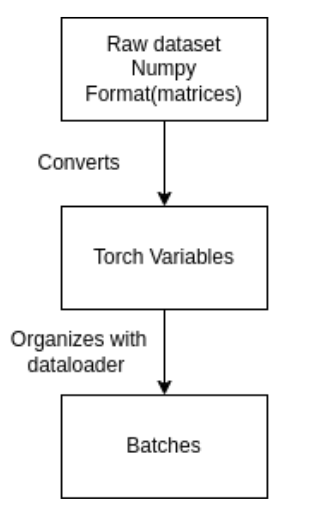
\includegraphics[width=0.3\textwidth]{training_pipeline.png}
    \caption{Training pipeline.}  
    \label{fig:training_pipeline}               
\end{figure}

\begin{itemize}
\item Once trained, the model can autonomously predict suitable visualizations for unseen datasets by leveraging the learned feature representations. The use of PyTorch ensures computational efficiency, with support for both CPU and GPU acceleration, while the modular architecture permits straightforward adaptation to varying input dimensions and classification tasks.
\end{itemize}


We ultimately concluded that, in summary, VizML's neural network training framework combines a high-capacity architecture with dynamic optimization strategies to achieve robust performance in visualization recommendation. The absence of significant gains from additional regularization implies that the model's default configuration effectively balances complexity and generalizability.
\subsubsection{Embedding Learning (KG4Vis)}

According to [2]:
\begin{itemize}
\item KG4Vis is a knowledge graph-based approach designed to automate visualization recommendations while maintaining explainability. At its core, it employs a knowledge graph (KG) to model relationships between various entities, such as dataset features, columns, and visualization design choices. To learn meaningful representations of these entities and their relationships, KG4Vis utilizes TransE embeddings, a knowledge graph embedding technique that maps entities and relations into a continuous vector space. This embedding method enables the system to infer new relationships and generate explainable recommendations by capturing structured patterns efficiently.

\item The learning process in KG4Vis involves several key steps. During training, the model optimizes its embeddings using gradient descent, adjusting vector representations to better fit the observed relationships in the knowledge graph. A key component of this optimization is the loss function, which ensures that correct relationships (i.e. valid triplets of head entity, relation, and tail entity) receive higher scores than incorrect ones. To improve learning robustness, KG4Vis employs negative sampling, a technique that generates false triplets, helping the model distinguish between valid and invalid relations. This approach improves generalization and scalability, making the system adaptable to various visualization recommendation tasks.

\item KG4Vis is implemented using PyTorch, which facilitates efficient computation and updating of knowledge graph embeddings. However, one limitation of this method is its computational cost, particularly when dealing with large-scale knowledge graphs. As the number of entities increases, the training process can become resource-intensive, and the quality of learned embeddings may degrade if the graph contains an excessive number of nodes.
\end{itemize}
The knowledge graph in KG4Vis consists of several types of nodes, each representing different aspects of the data and visualization process. These include:

\begin{itemize}

\item Data columns, which represent individual columns within datasets;

\item  Discretized continuous data features, where continuous attributes are divided into intervals for analysis;

\item Categorical data features, representing discrete attributes;

\item Visualization design choices, denoting different visualization types and their configurations.
\end{itemize}
The relationships between these nodes are captured through edges, which define how entities interact. For instance, edges connect data columns to their respective features (e.g., data type, name), while other edges link data features to appropriate visualization choices, ensuring that certain data characteristics align with optimal visual encodings. Additionally, some edges directly associate data columns with visualization choices, specifying how columns should be used in different chart types.
\medskip
\par
We then found that, unlike some other recommendation systems, KG4Vis does not incorporate reinforcement learning (RL) to dynamically adjust its knowledge graph based on feedback. Instead, it relies solely on embedded learning to infer recommendations, which remain static once learned. Although this approach ensures efficiency and explainability, it does not adapt over time through trial-and-error mechanisms, which could potentially refine recommendations based on user interactions.


\subsection{Visualization Recommendation Process}

We found that the visualization recommendation process differs significantly between the two models compared in this study. Both aim to suggest appropriate visualizations; however, they employ fundamentally different approaches to arrive at their recommendations.

\subsubsection{VizML’s Direct Prediction}

According to [1]:
\begin{itemize}
\item VizML employs a data-driven approach for visualization recommendation, operating through direct prediction mechanisms. The model analyzes the characteristics of the input data and directly predicts the visualization design choices without explicitly modeling the reasoning process. \par 
\end{itemize}
This approach leverages deep neural networks trained on large datasets of visualization examples.
The direct prediction process follows these steps:
\begin{itemize}
\item Feature extraction from input data, including statistical properties, data types, and distribution characteristics
\item Processing these features through neural network training
\item Outputting probability scores for different visualization types and encoding options
\item Selecting the visualization design with the highest probability score
\end{itemize}
\medskip
We found that VizML's strengths lie in its ability to identify complex patterns between data characteristics and visualization choices based on statistical correlations observed in the training data. However, this approach significantly decreases possible insight into why specific recommendations are made beyond numeric probability scores.

\subsubsection{KG4Vis’ Explanation-Based Recommendations}

According to [2]:
\begin{itemize}
\item KG4Vis adopts a knowledge-based approach centered on explanation and reasoning. The model constructs recommendations through a structured knowledge graph that represents relationships between data attributes, visualization designs, and design principles. \par
\end{itemize}
KG4Vis generates recommendations through:
\begin{itemize}
\item Analyzing input data and mapping its characteristics to entities in the knowledge graph
\item Traversing the knowledge graph using embedding-based algorithms\linebreak (TransE) to identify related visualization concepts
\item Applying rule-based reasoning to evaluate potential visualization options
\item Generating explanations that connect input data characteristics to visualization suggestions through explicit reasoning chains
\end{itemize}
\medskip
We found that:
\begin{itemize}
\item This approach aims to increase interpretability and transparency in the recommendation process. Rather than simply suggesting a visualization type, KG4Vis provides justifications based on established design principles and domain knowledge encoded in its knowledge graph.
\item The embedding learning component allows the model to capture semantic relationships between visualization concepts, allowing more thought-out recommendations that consider multiple factors simultaneously.
\end{itemize}
The following Fig. 3 represents examples of KG4Vis' graphs.

\Needspace{11\baselineskip}

\begin{figure}[h]
    \centering
    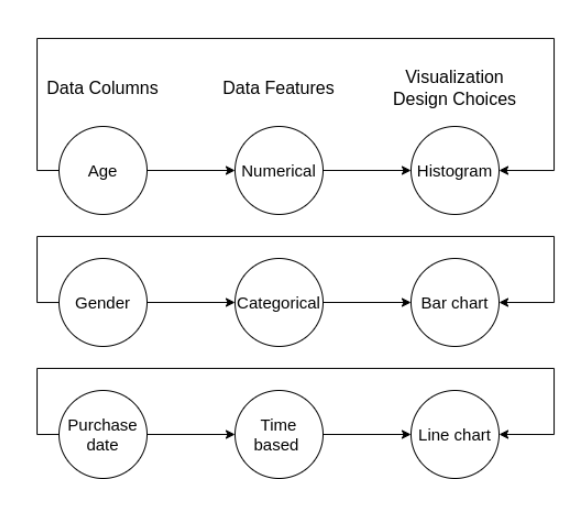
\includegraphics[width=0.9\textwidth]{Graphs_examples.png}
    \caption{Examples of Graphs on KG4Vis model.}  
    \label{fig:graficos_exemplo}               
\end{figure}

\subsubsection{Models' Summary}

\begin{table}[H]
    \centering
    \caption{Models' Comparison.}
    \begin{tabular}{|p{2cm}|p{4.4cm}|p{4.4cm}|}
    \hline
    \ & \textbf{VizML} & \textbf{KG4Vis} \\
    \hline
    Core  \newline Approach & Machine learning-based approach using neural networks trained on large corpus of dataset-visualization pairs from Plotly Community Feed & Knowledge graph-based approach using TransE embedding technique to model relationships between data features, columns, and visualization design choices \\
    \hline
    Explainability & Limited explainability - neural networks work as "black box" models, though feature importances can be extracted from baseline models & High explainability - generates semantically meaningful rules that can be traced back to understand why specific visualizations are recommended \\
    \hline
    Extensibility & Requires retraining models with new data; limited by the original training corpus structure and visualization types & Easily extensible by adding new entities, relations, and triplets to the knowledge graph without complete retraining \\
    \hline
    Technology \newline Requirements & - Large-scale dataset (1M+ dataset-visualization pairs)\newline- Neural network training infrastructure\newline- PyTorch/deep learning frameworks\newline- Significant computational requirements for training & - Knowledge graph construction tools\newline- TransE embedding learning\newline- Moderate computational requirements\newline- MDLP discretization for continuous features \\

    
    \hline
    \end{tabular}
    \end{table}

\subsection{Technology Stack}

Both VizML and KG4Vis require specific Python environments and associated libraries to support their implementation. VizML is built on Python 3.7.3, relying heavily on data-science and machine-learning packages for model training, feature extraction, and visualization. Core packages include NumPy, Pandas, Matplotlib, Scikit-learn, and PyTorch, as well as additional utilities for handling time-series, text processing, and imbalanced datasets. The full list of packages and their versions is shown in Table 3.

\begin{table}[h!]
    \centering
    \caption{Library Versions.}
    \begin{tabular}{|l|l|}
    \hline
    \textbf{Name} & \textbf{Version} \\
    \hline
    cycler       & 0.10.0 \\
    editdistance & 0.5.3  \\
    kiwisolver   & 1.1.0  \\
    matplotlib   & 3.0.3  \\
    numpy        & 1.16.3 \\
    pandas       & 0.24.2 \\
    pyparsing    & 2.4.0  \\
    python-dateutil & 2.8.0  \\
    pytz        & 2019.1 \\
    scikit-learn & 0.20.3 \\
    scipy       & 1.2.1  \\
    six         & 1.12.0 \\
    seaborn     &   \\
    IPython     &  \\
    pytorch   &   \\
    imbalanced-learn &  \\
    \hline
    \end{tabular}
    \end{table}

\vspace{40cm}

\noindent In contrast, KG4Vis is implemented using Python 3.7.9, leveraging a more compact library stack centered on knowledge-graph representation and embedding techniques. Its requirements focus on NumPy, Pandas, Scikit-learn, PyTorch, and utility packages like tqdm for efficient progress tracking. These dependencies, shown in Table 4, reflect its emphasis on relational learning and graph-based reasoning rather than end-to-end neural network training.

\begin{table}[H]
    \centering
    \caption{Library Versions.}
    \begin{tabular}{|l|l|}
    \hline
    \textbf{Name} & \textbf{Version} \\
    \hline
    scikit-learn & 0.21.0 \\
    numpy        & 1.16.3 \\
    editdistance & 0.5.3  \\
    pandas       & 0.24.2 \\
    pytorch   &   1.7.0\\
    tqdm &   4.66.4\\
    \hline
    \end{tabular}
    \end{table}


\subsection{Dataset}

According to [1] and [2]:
\begin{itemize}
\item The dataset was retrieved from the KG4Vis GitHub repository. It is the same dataset used for VizML and was originally sourced from various datasets available on Plotly, according to [1] and [2].
\end{itemize}
\vspace{1.0cm}

It consists of rows corresponding to unique visualizations or charts. Each row contains two main columns:
\begin{itemize}
\item \texttt{fid}: A unique identifier for each visualization (e.g. xiemei:82, Wini:4).

\item \texttt{chart\_data}: A JSON-like structure containing the configuration and metadata for the visualization.
\end{itemize}

The dataset includes a variety of visualization types, such as scatter plots, line charts, bar charts, histograms, heatmaps, and fitted curves. Each chart\_data entry contains detailed properties for the visualization, including the chart type (e.g. scatter, bar, heatmap), mode (e.g., markers, lines, lines+markers), name (a label or title for the data series), marker properties (e.g., color, size, symbol), and line properties (e.g., color, width, dash style).
\medskip
\par
For the purpose of model development and evaluation, the dataset was split into training and testing subsets.

    
\subsection{Training}

This section details the training process for both VizML and KG4Vis models, covering dataset preparation, feature extraction, and model training. The subsections are structured as follows:

\begin{itemize}
    \item \textbf {5.6.1 Dataset Build:} Describes the preprocessing steps to convert, clean, and prepare the raw dataset for analysis.
    \item \textbf {5.6.2 VizML Feature Extraction:} Explains how numerical features are extracted and normalized for neural network input.
    \item \textbf {5.6.3 KG4Vis Feature Extraction:} Outlines the transformation of raw data into graph-structured representations for knowledge graph construction.
    \item \textbf {5.6.4 VizML Model Training:} Covers the neural network architecture, optimization, and training pipeline for VizML.
    \item \textbf {5.6.5 KG4Vis Model Training:} Details the embedding learning process and knowledge graph optimization for KG4Vis.
    
\end{itemize}


\subsubsection{ Dataset Build}
The following steps describe the preprocessing steps used to convert the raw dataset described in the previous section into a dataset that can be used for VizML training. These steps are not necessary for the KG4Vis project, since it uses the raw dataset for feature extraction and model training.

Prior to conducting any analysis, the dataset must undergo a series of preprocessing steps to ensure compatibility and data integrity. The initial phase involves converting the dataset from Comma-Separated Values (CSV) format to Tab-Separated Values (TSV) format. This conversion is performed to mitigate potential parsing conflicts arising from embedded commas within the data fields. The transformation is executed using the following AWK command:
\begin{verbatim}
awk 'BEGIN { FS=","; OFS="\t" } {$1=$1; print}' raw_data_all.csv
> plot_data.tsv 
\end{verbatim}

Following the format conversion, the dataset undergoes a data cleaning procedure to eliminate invalid and redundant entries. This step is crucial to maintain the consistency and reliability of subsequent analyses. The cleaning process consists of two sequential operations, executed within the data\_cleaning directory:

\begin{verbatim}
    python remove_charts_without_all_data.py
\end{verbatim}
This script filters out visualization records that lack complete data attributes, ensuring that only fully specified entries are retained.

\begin{verbatim}
    python remove_duplicate_charts.py
\end{verbatim}
This step identifies and removes duplicate visualization entries, preventing redundancy and potential bias in downstream analyses.

Once the dataset has been cleaned, the next phase involves feature extraction, which transforms raw data into structured, machine-interpretable representations. This process is executed by running the following command within the feature\_extraction directory:
\begin{verbatim}
    python extract.py
\end{verbatim}

The feature extraction module systematically parses the dataset, identifying and encoding relevant attributes that will later inform visualization recommendations. This structured preprocessing pipeline ensures that the input data adheres to the required format and quality standards before further computational analysis and is illustrated in the following Fig. 4.

\begin{figure}[h]
    \centering
    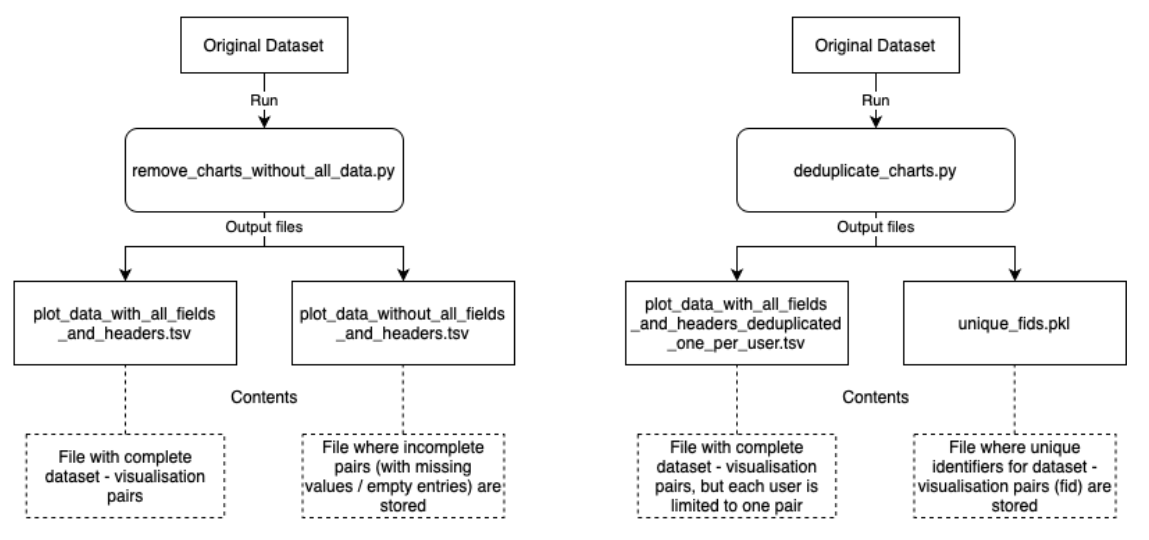
\includegraphics[width=1\textwidth]{Data_Cleaning.png}
    \caption{Data Cleaning Pipeline for VizML.}  
    \label{fig:datacleaning}               
\end{figure}

\vspace{10cm}
\subsubsection{ VizML Feature Extraction}
According to [1], VizML performs feature extraction by analyzing dataset columns and quantifying their statistical and structural properties. Specifically, it computes 841 features per dataset, which include metrics such as mean, standard deviation, skewness, kurtosis, and missing value ratios. These features are derived from individual columns and across column pairs, enabling the model to capture relationships within the dataset. The extracted features are then normalized and converted into numerical vectors, forming a feature vector that serves as input to the neural network. This process is entirely automatic and allows the model to generalize across a wide range of dataset types.

\subsubsection{ KG4Vis Feature Extraction}
According to [2], KG4Vis leverages the same raw dataset-visualization pairs used in VizML but represents the extracted information in a different format. Instead of computing numerical feature vectors, KG4Vis encodes dataset characteristics as nodes in a knowledge graph. For example, a column's data type ("Categorical data") is represented as a node, and its relationship to a recommended chart ("Bar chart") is encoded as an edge. This transformation from raw data to graph-structured representation allows the system to explicitly model semantic relationships between features and visualization types. The graph structure enhances both interpretability and extensibility, as new features and chart types can be integrated without retraining the system.

\subsubsection{ VizML Model Training}
According to [1], VizML uses a supervised deep learning approach, training a fully connected feedforward neural network using the extracted 841-dimensional feature vectors and their corresponding chart labels. The network is trained using PyTorch, where input vectors are processed in batches, passed through hidden layers, and updated through backpropagation to minimize categorical cross-entropy loss. This training process is computationally intensive, often requiring GPU acceleration and large memory capacity (RAM/VRAM) to handle large datasets. Once trained, the model can predict the most suitable chart type for new datasets via a single forward pass, achieving high-speed inference at the cost of reduced explainability.

\subsubsection{ KG4Vis Model Training}
According to [2], KG4Vis does not rely on traditional classification training but instead trains vector embeddings for each node and relation in the knowledge graph. Using TransE embeddings, KG4Vis learns to represent semantic relationships in vector space such that if A is related to B through R, the embedding satisfies the approximation $A + R \approx B$. This training is conducted using PyTorch, which manages both the computation of the embedding vectors and the optimization of the model through stochastic gradient descent. The trained embeddings allow KG4Vis to perform embedding-based inference, meaning it can recommend the most contextually appropriate visualization and explain the reasoning behind the choice. Additionally, this setup allows the model to infer missing links in the graph, dynamically expanding its knowledge without retraining from scratch.

\subsection{Tests}
When testing, we evaluate the generalizability of each model. \par
\vspace{10pt}
\noindent For VizML, during its testing, we found several problems with the model's implementation. Due to missing code and system-level implementation issues beyond the scope of our expertise, we were unable to execute certain components of the model training pipeline to full capacity. \par
To avoid these technical limitations, we sought the help of generative AI to fill the gaps in the code and fix most errors; however, no progress was able to be made and we continued to have the same recurring difficulties. \par
Seeing as we had found another model and had been interacting with it so far, we decided to stop attempting to run VizML and dedicated our full focus to KG4Vis. \par
\vspace{10pt}
\noindent For the KG4Vis project, we trained the knowledge graph embedding model using TransE with various parameter configurations to optimize computational efficiency while trying to maintain model quality. \par
Initially, the evaluation was carried out using a configuration constrained by hardware limitations, specifically, the available system memory. Due to memory-related crashes at higher batch sizes, we iteratively halved this parameter, settling on a batch size of 32 as the largest viable value that allowed training to be completed successfully.\par
Subsequently, a second configuration was tested, which allowed training with the full batch size of 1024. However, this configuration did not support CUDA acceleration due to the absence of a NVIDIA GPU, relying on CPU computation. \par
Both configurations used hidden dimensions ranging from 500 to 1000, increasing in steps of 100. This range was selected to study how the representational capacity of the model embeddings affects performance. Larger hidden dimensions can capture more complex patterns, potentially improving accuracy at the cost of an increase in computational cost and training time. \par
\vspace{0.3cm}
\noindent\textbf{Configuration summary:}
\begin{itemize}
    \item \textbf{Configuration 1:} Batch size = 32, Hidden dimensions = 500--1000 (step of 100), ran on Lenovo's Legion Pro 5, on a Windows 11 system, equipped with an AMD Ryzen 9 7945HX processor (2.50 GHz, 32 cores), 32GB of installed RAM and an NVIDIA GeForce RTX 4070 Laptop GPU with 8GB dedicated VRAM. However, training was performed within a Windows Subsystem for Linux (WSL) environment, which utilized Python 3.7.17 with PyTorch 1.7.0 and CUDA 12.9 support through NVIDIA driver version 576.40 but only had access to 15GB of the total system memory. Due to memory management constraints within the WSL, batch size had to be limited to 32 (crashes at higher sizes).
    \item \textbf{Configuration 2:} Batch size = 1024, same hidden dimensions, running on Apple M2 Max (32 GB RAM), no CUDA acceleration available, computation performed on CPU with low power mode on.
\end{itemize}

Model performance was assessed using standard knowledge graph metrics, including Hit@k and Mean Reciprocal Rank (MRR). These metrics evaluate how effectively the embedding model ranks relevant visualizations when presented with user input or data characteristics. Training convergence was monitored through loss values.

\subsection{Comparative Analysis and Discussion of KG4Vis}

\subsubsection{Scalability}
To evaluate the model's scalability, we measured the total training compared for each of the hidden dimension values, as shown in Fig./Table 5 and 6.

\vspace{4.0cm}
\textbf{Configuration 1}

\begin{figure}[H]
    \centering
    \includegraphics[width=1\textwidth]{configuration_1/dim_time.pdf}
    \caption{Total training time for different values of Hidden Dimension (Configuration 1).}  
    \label{fig:time_hidden_dim_evolution_c1}               
\end{figure}

\Needspace{7\baselineskip}

\begin{table}[h]
\centering
\caption{Numerical values of total training time for different values of Hidden Dimension (Configuration 1).}
\begin{tabular}{|c|c|}
\hline
Hidden Dimension & Training Time (s)\\
\hline
500  & 800\\
600  & 933\\
700  & 1075\\
800  & 1220\\
900  & 1362\\
1000  & 1504\\
\hline
\end{tabular}
\label{tab:time_hidden_dim_evolution_table_c1}
\end{table}

We noticed that for this configuration, as shown in Table 5, the relation between the hidden dimension and the training time closely follows a linear relation of $m \approx 1,54$. This indicates that training time increases proportionally with model complexity, suggesting efficient and consistent computational scaling as dimensionality grows.

\vspace{1.8cm}
\textbf{Configuration 2}

\begin{figure}[H]
    \centering
    \includegraphics[width=1\textwidth]{configuration_2/dim_time.pdf}
    \caption{Total training time for different values of Hidden Dimension (Configuration 2).}  
    \label{fig:time_hidden_dim_evolution_c2}               
\end{figure}

\Needspace{7\baselineskip}

\begin{table}[h]
\centering
\caption{Numerical values of total training time for different values of Hidden Dimension (Configuration 2).}
\begin{tabular}{|c|c|}
\hline
Hidden Dimension & Training Time (s)\\
\hline
500  & 5173\\
600  & 5897\\
700  & 14689\\
800  & 16787\\
900  & 19662\\
1000  & 21723\\
\hline
\end{tabular}
\label{tab:time_hidden_dim_evolution_table_c2}
\end{table}

Configuration 2 has a much longer training time overall compared to configuration 1, as we can observe from the results in Table 6, mainly due to the missing CUDA acceleration. The graph shows a drastic increase in training time between 600 and 700 hidden dimensions. \par
\begin{itemize}
\item For hidden dimensions between 500 and 600, the relation is that of $m \approx 10,09$;
\item For hidden dimensions between 700 and 1000, the relation is that of $m \approx 21,38$. 
\end{itemize}
This difference suggests that different internal computational behaviors may be triggered at different hidden dimension thresholds, such as memory management or other types of hardware-dependent optimizations. 

\subsubsection{Performance}
To evaluate the model's performance, we analyzed the overall evolution of the metrics over the different hidden dimensions, as shown in Fig./Table 7 and 8.

\vspace{0.3cm}
\textbf{Configuration 1}
\begin{figure}[H]
    \centering
    \includegraphics[width=1\textwidth]{configuration_1/measured_metrics_hidden_dim.pdf}
    \caption{Metrics evolution for different values of Hidden Dimension (Configuration 1).}  
    \label{fig:metrics_hidden_dim_c1}               
\end{figure}

\Needspace{7\baselineskip}

\begin{table}[h]
\centering
\caption{Metrics for different values of Hidden Dimension (Configuration 1).}
\begin{tabular}{|c|c|c|c|}
\hline
Hidden Dimension & Hits@2 (\%) & Axis Accuracy (\%) & Mean Rank \\
\hline
500  & 71.6 & 61.0 & 2.06\\
600  & 49.6 & 38.9 & 3.06\\
700  & 42.7 & 38.9 & 3.54\\
800  & 7.0 & 38.7 & 4.07\\
900  & 42.8 & 44.5 & 3.35\\
1000  & 38.9 & 61.0  & 2.67\\
\hline
\end{tabular}
\label{tab:metrics_hidden_dim_table_c1}
\end{table}

For a batch size of 32, we obtained the best results for a hidden dimension of 500, as is seen in Table 7. Contrary to what is expected, reducing the size of each batch from 1024 (default value) using a lower hidden dimension proved to be beneficial for the model. We also noticed that for a hidden dimension of 800, the results were significantly worse compared to the other values used. Since only the hidden dim changed across different executions, this could suggest that using a batch size of 32 and a hidden dimension of 800 caused the model to overfit or enter a saturated regime, leading to ineffective learning.

\vspace{0.5cm}
\textbf{Configuration 2}
\begin{figure}[H]
    \centering
    \includegraphics[width=1\textwidth]{configuration_2/measured_metrics_hidden_dim.pdf}
    \caption{Metrics evolution for different values of Hidden Dimension (Configuration 2).}  
    \label{fig:metrics_hidden_dim_c2}               
\end{figure}

\Needspace{7\baselineskip}

\begin{table}[h]
\centering
\caption{Metrics for different values of Hidden Dimension (Configuration 2).}
\begin{tabular}{|c|c|c|c|}
\hline
Hidden Dimension & Hits@2 (\%) & Axis Accuracy (\%) & Mean Rank \\
\hline
500  & 73.9 & 75.4 & 2.00\\
600  & 74.5 & 74.8 & 1.98\\
700  & 73.2 & 75.9 & 2.00\\
800  & 68.5 & 76.9 & 2.10\\
900  & 71.8 & 77.2 & 2.08\\
1000  & 62.0 & 75.8  & 2.32\\
\hline
\end{tabular}
\label{tab:metrics_hidden_dim_table_c2}
\end{table}

Similarly to the previous configuration, the best results were obtained at a lower hidden dimension, specifically 600, seen in Table 8. This suggests that at higher batch sizes, smaller hidden dimensions may lead to better generalization by reducing model complexity while still maintaining sufficient representational capacity. Higher hidden dimensions (e.g. 800-1000) likely introduced excess capacity, which may have led to overfitting. Additionally, lower hidden dimensions train faster and may benefit from improved gradient stability and a reduced risk of overfitting, resulting in a better generalization, observed by highest Hits@2 and the lowest Mean Rank. \par
A performance drop is also observed in a hidden dimension of 800, although less pronounced than in the previous configuration. This consistency across different batch sizes suggests that, for this particular model architecture, a hidden dimension of 800 may correspond to a suboptimal capacity regime, potentially leading to inefficient gradient flow or representational instability. 

\subsubsection{Accuracy}
To evaluate the model's accuracy, we analyzed the evolution of the Hits@2 and Axis Accuracy metrics across the different hidden dimensions, as shown in Fig./Table 9 and 10.

\vspace{0.3cm}
\textbf{Configuration 1}
\begin{figure}[H]
    \centering
    \includegraphics[width=1\textwidth]{configuration_1/accuracy_metrics.pdf}
    \caption{Hits@2 and Axis Accuracy percentages for different values of Hidden Dimension (higher is better) (Configuration 1).}  
    \label{fig:accuracy_metrics_c1}               
\end{figure}

\Needspace{7\baselineskip}

\begin{table}[h]
\centering
\caption{Hits@2 and Axis Accuracy for different values of Hidden Dimension (Configuration 1).}
\begin{tabular}{|c|c|c|}
\hline
Hidden Dimension & Hits@2 (\%) & Axis Accuracy (\%)\\
\hline
500  & 71.6 & 61.0\\
600  & 49.6 & 38.9\\
700  & 42.7 & 38.9\\
800  & 7.0 & 38.7\\
900  & 42.8 & 44.5\\
1000  & 38.9 & 61.0\\
\hline
\end{tabular}
\label{tab:accuracy_metrics_table_c1}
\end{table}
The evolution of Hits@2 and Axis Accuracy aligns with the performance trends discussed above. As shown in Table 9, the highest accuracy metrics were observed at a hidden dimension of 500, while a clear degradation was observed at 800. These results reinforce the conclusion drawn regarding the capacity and generalization of the model.

\vspace{0.5cm}
\textbf{Configuration 2}
\begin{figure}[H]
    \centering
    \includegraphics[width=1\textwidth]{configuration_2/accuracy_metrics.pdf}
    \caption{Hits@2 and Axis Accuracy percentages for different values of Hidden Dimension (higher is better) (Configuration 2).}  
    \label{fig:accuracy_metrics_c2} 
\end{figure}

\begin{table}[h]
\centering
\caption{Hits@2 and Axis Accuracy for different values of Hidden Dimension (Configuration 2).}
\begin{tabular}{|c|c|c|}
\hline
Hidden Dimension & Hits@2 (\%) & Axis Accuracy (\%)\\
\hline
500  & 73.9 & 75.4\\
600  & 74.5 & 74.8\\
700  & 73.2 & 75.9\\
800  & 68.5 & 76.9\\
900  & 71.8 & 77.2\\
1000  & 62.0 & 75.8\\
\hline
\end{tabular}
\label{tab:accuracy_metrics_table_c2}
\end{table}
Hits@2 and Axis Accuracy remained relatively high in most dimensions, with the best values at a hidden dimension of 600, observed in Table 10. These results support the earlier observation that smaller hidden dimensions tend to generalize better at larger batch sizes.

\subsubsection{Precision}
To evaluate the model's precision, we analyzed the evolution of the Mean Rank metric across the different hidden dimensions, as shown in Fig./Table 11 and 12.

\vspace{0.3cm}
\textbf{Configuration 1}
\begin{figure}[H]
    \centering
    \includegraphics[width=1\textwidth]{configuration_1/precision_metrics.pdf}
    \caption{Mean Rank for value different values of Hidden Dimension (lower is better) (Configuration 1).}  
    \label{fig:precision_metrics_c1}               
\end{figure}

\Needspace{7\baselineskip}

\begin{table}[h]
\centering
\caption{Mean Rank for different values of Hidden Dimension (Configuration 1).}
\begin{tabular}{|c|c|}
\hline
Hidden Dimension & Mean Rank \\
\hline
500  & 2.06\\
600  & 3.06\\
700  & 3.54\\
800  & 4.07\\
900  & 3.35\\
1000  & 2.67\\
\hline
\end{tabular}
\label{tab:precision_metrics_table_c1}
\end{table}

Mean Rank values also followed the trend discussed previously, where the best value was observed at a hidden dimension of 500, shown in Table 11. The sharp increase in Mean Rank at 800 confirms the degraded performance, highlighting reduced precision in ranking predictions.

\vspace{0.5cm}
\textbf{Configuration 2}
\begin{figure}[H]
    \centering
    \includegraphics[width=1\textwidth]{configuration_2/precision_metrics.pdf}
    \caption{Mean Rank for value different values of Hidden Dimension (lower is better) (Configuration 2).}  
    \label{fig:precision_metrics_c2}               
\end{figure}

\Needspace{7\baselineskip}

\begin{table}[h]
\centering
\caption{Mean Rank for different values of Hidden Dimension (Configuration 2).}
\begin{tabular}{|c|c|}
\hline
Hidden Dimension & Mean Rank \\
\hline
500  & 2.00\\
600  & 1.98\\
700  & 2.00\\
800  & 2.10\\
900  & 2.08\\
1000  & 2.32\\
\hline
\end{tabular}
\label{tab:precison_metrics_table_c2}
\end{table}

As observed earlier and in Table 12, the Mean Rank was better at a hidden dimension of 600. The gradual increase beyond this point supports the argument that larger hidden dimensions may hurt precision due to increased model complexity and potential overfitting.


%\subsection{Architecture and technologies}

%Architecture and technologies used and their justification, technical diagrams drawn up, technical difficulties encountered and their resolution, etc.





%\subsection{Developed solution}

%Present the developed solution from the user's point of view, with the help of screenshots.

%\subsection{Validation}

%Description of the validation of the developed solution (e.g. experimental evaluation results, tests carried out, feedback from users or experts, etc.)
